%auto-ignore

\section{Related Work}
There is a long history of pre-training general language representations, and we briefly review the most widely-used approaches in this section.


\subsection{Unsupervised Feature-based Approaches}
Learning widely applicable representations of words has been an active area of research for decades, including non-neural~\cite{brown-etal:1992:_class, ando-zhang:2005, blitzer-mcdonald-pereira:2006:_domain} and neural~\cite{mikolov-etal:2013, pennington-socher-manning:2014:_glove} methods. Pre-trained word embeddings are an integral part of modern NLP systems, offering significant improvements over embeddings learned from scratch~\cite{turian-ratinov-bengio:2010:_word_repres}. To pre-train word embedding vectors, left-to-right language modeling objectives have been used~\cite{minh09}, as well as objectives to  discriminate correct from incorrect words in left and right context~\cite{mikolov-etal:2013}.

These approaches have been generalized to coarser granularities, such as sentence embeddings~\cite{kiros-etal:2015:_skip, logeswaran2018an} or paragraph embeddings~\cite{le-mikolov:2014:_distr}. To train sentence representations, prior work has used objectives to rank candidate next sentences  \cite{DBLP:journals/corr/JerniteBS17, logeswaran2018an},  left-to-right generation of next sentence words given a representation of the previous sentence~\cite{kiros-etal:2015:_skip}, or denoising auto-encoder derived objectives~\cite{hill16}.

%
\begin{figure*}[t!]
%\small
\begin{center}
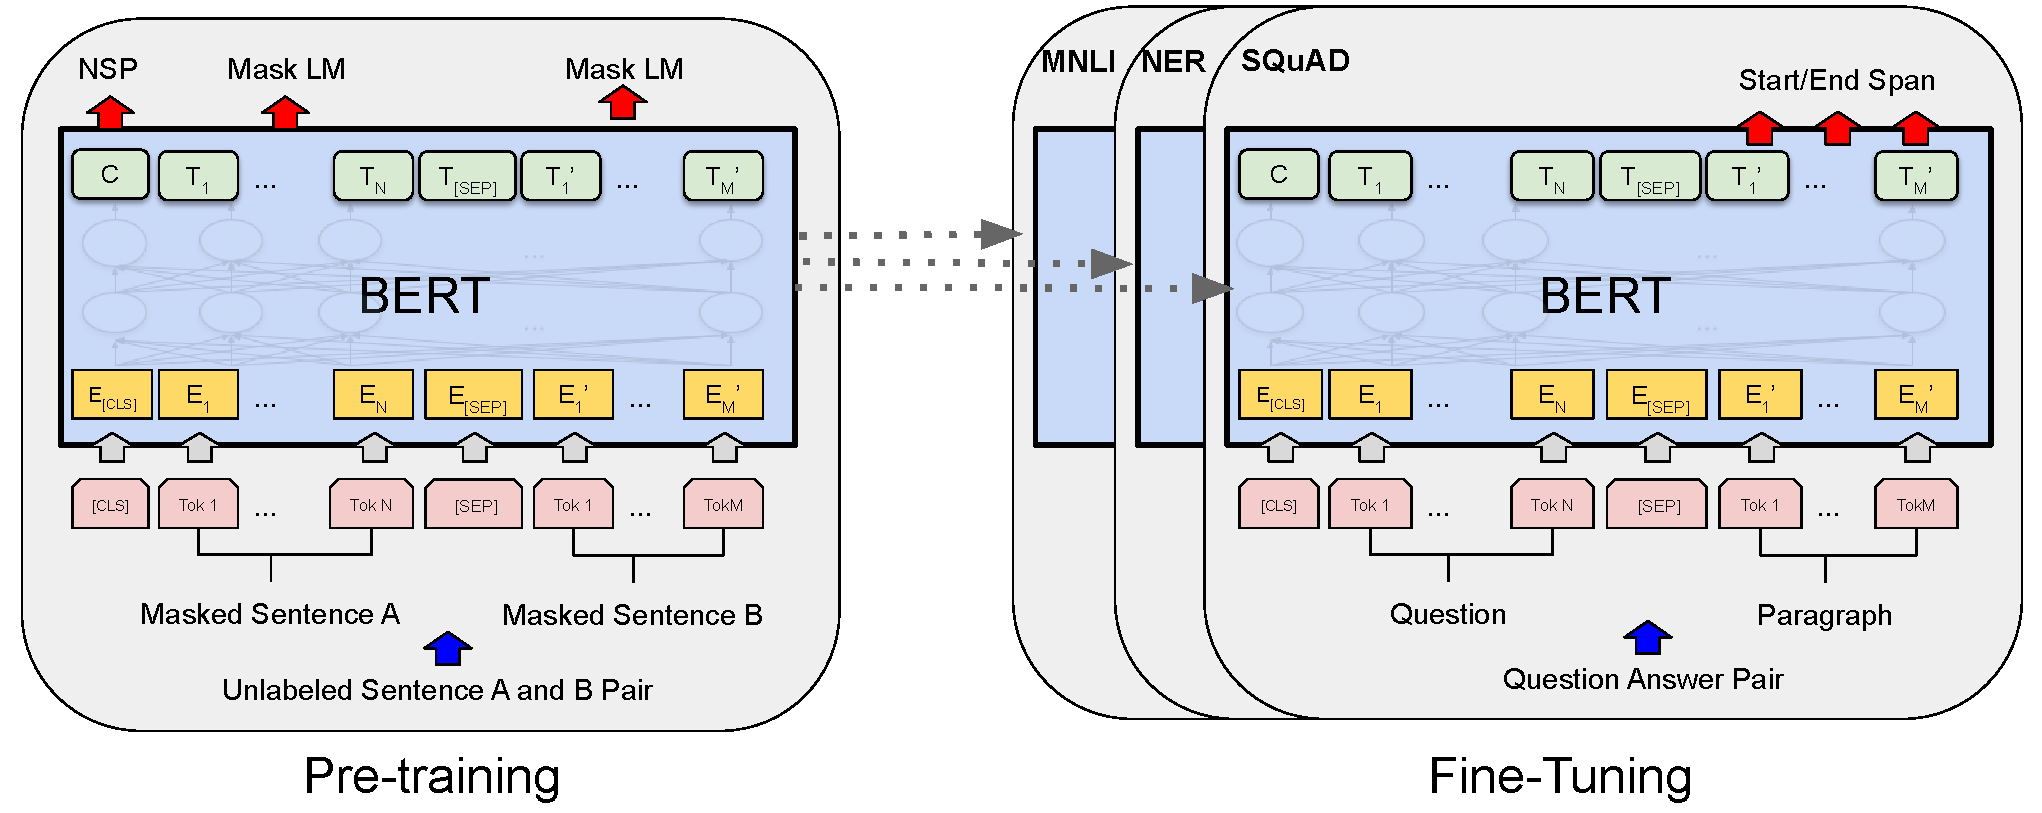
\includegraphics[width=1\textwidth]{BERT_Overall.pdf}
\end{center}
\caption{Overall pre-training and fine-tuning procedures for BERT. Apart from output layers, the same architectures are used in both pre-training and fine-tuning. The same pre-trained model parameters are used to initialize models for different down-stream tasks.  During fine-tuning, all parameters are fine-tuned. {\tt [CLS]} is a special symbol added
in front of every input example, and {\tt [SEP]} is a special separator token (e.g. separating  questions/answers).}
\label{fig:bert_overall}
\end{figure*}
%



ELMo and its predecessor~\cite{peters-etal:2017:_semi, peters-etal:2018:_deep} generalize traditional word embedding research along a different dimension. They extract \emph{context-sensitive} features from a left-to-right and a right-to-left language model. The contextual representation of each token is the concatenation of the left-to-right and right-to-left representations. When integrating contextual word embeddings with existing task-specific architectures, ELMo advances the state of the art for several major NLP benchmarks~\cite{peters-etal:2018:_deep} including question answering~\cite{rajpurkar-etal:2016:_squad}, sentiment analysis~\cite{socher-etal:2013:_recur}, and named entity recognition~\cite{tjong-de:2003}.
\citet{melamud2016context2vec} proposed learning contextual representations through a task to predict a single word from both left and right context
using LSTMs. Similar to ELMo, their model is feature-based and not deeply bidirectional. 
\citet{fedus2018maskgan} shows that the cloze task can be used to improve the robustness of text generation models. 




\subsection{Unsupervised Fine-tuning Approaches}

As with the feature-based approaches, the first works in this direction only pre-trained word embedding parameters from unlabeled text ~\cite{collobert-weston:2008}.  

More recently, sentence or document encoders which produce contextual token representations have been pre-trained from unlabeled text and fine-tuned for a supervised downstream task~\cite{dai-le:2015:_semi, howard-ruder:2018, radford-etal:2018}.  The advantage of these approaches is that few parameters need to be learned from scratch. At least partly due to this advantage, OpenAI GPT~\cite{radford-etal:2018} achieved previously state-of-the-art results on many sentence-level tasks from the GLUE benchmark~\cite{wang-etal:2018:_glue}.  Left-to-right language modeling and auto-encoder objectives have been used for pre-training such models~\cite{howard-ruder:2018, radford-etal:2018,dai-le:2015:_semi}.





\subsection{Transfer Learning from Supervised Data}

There has also been work showing effective transfer from supervised tasks with large datasets, such as natural language inference~\cite{conneau-EtAl:2017:EMNLP2017} and machine translation~\cite{mccann-etal:2017:_learn_trans}. 
Computer vision research has also demonstrated the importance of transfer learning from large pre-trained models, where an effective recipe is to fine-tune models pre-trained with ImageNet~\cite{imagenet_cvpr09, yosinski2014transferable}. 



